\begin{center}
  \textsf{Листок 1.}
\end{center}
\vspace{0.01cm}
\nopagebreak[2]

\taskpic{ На диаграмме изображены два цикла, которые проводят с
  одноатомным идеальным газом: $1-2-3-1$ и $1-3-4-1$. У какого из
  циклов КПД больше и во сколько раз?}{
  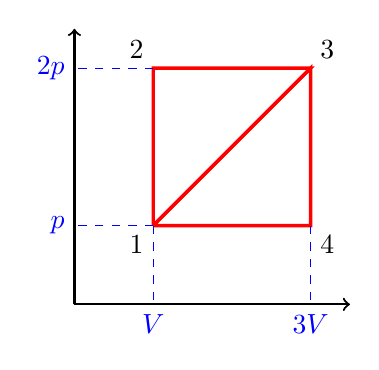
\begin{tikzpicture}
    \draw[thick,->] (0,0) -- (0,3.5);
    \draw[thick,->] (0,0) -- (3.5,0);
    \coordinate (a) at (1,1);
    \coordinate (b) at (3,1);
    \coordinate (c) at (3,3);
    \coordinate (d) at (1,3);
    \draw[very thick,red] (a) -- (b) -- (c) -- (a);
    \draw[very thick,red] (a) -- (d) -- (c) -- (a);
    \draw (a) node[below left] {1};
    \draw (b) node[below right] {4};
    \draw (c) node[above right] {3};
    \draw (d) node[above left] {2};
    \draw[blue,dashed] (a) -- ++(0,-1) node[below] {$V$};
    \draw[blue,dashed] (b) -- ++(0,-1) node[below] {$3V$};
    \draw[blue,dashed] (a) -- ++(-1,0) node[left] {$p$};
    \draw[blue,dashed] (d) -- ++(-1,0) node[left] {$2p$};
\end{tikzpicture}  
}

\taskpic{ На расстоянии $d$ от заземленной сферы радиуса $R$ находится
  заряд $q$. Найти потенциал в любой точке пространства.  }{
  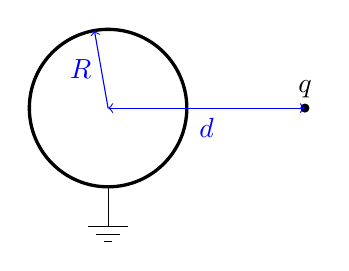
\begin{tikzpicture} 
    \draw[very thick] (1,2) circle (1);
    \draw[blue,->] (1,2) --++(100:1) node[midway, left] {$R$};
    \draw[fill=black] (3.5,2) circle (0.05) node[above] {$q$}; 
    \draw[blue,<->] (1,2) -- (3.5,2) node[midway,below] {$d$};
    \draw (1,1) -- (1,0.5);
    \draw (0.75,0.5) -- ++(0.5,0);
    \draw (0.85,0.4) -- ++(0.3,0);
    \draw (0.95,0.3) -- ++(0.1,0);
\end{tikzpicture}  
}

\task{ Планету массой $M$ и радиуса $r$ окружает атмосфера постоянной
  плотности, состоящая из газа с молярной массой $\mu$. Определите
  температуру $T$ атмосферы на поверхности планеты, если толщина
  атмосферы $h$ $(h\ll r)$.  }

\task{ Нелинейный двухполюсник имеет квадратичную ВАХ: напряжение
  между его выводами пропорционально квадрату текущего через него
  тока.  Двухполюсник подключают к батарейке с напряжением $U$
  последовательно с вольтметром, при этом вольтметр показывает
  половину напряжения батарейки. Параллельно двухполюснику подключают
  еще один такой же вольтметр. Найти показания вольтметров. Внутреннее
  сопротивление батарейки считать малым.  }

\task{ Цепь содержит огромное количество звеньев, каждое звено состоит
  из резистора и двух вольтметров. Все вольтметры в цепи
  одинаковы, сопротивления всех резисторов цепи равны между собой.
  Цепь подключают к батарейке, при этом первые два вольтметра
  показывают напряжение $6V$ и $4V$. Найти показания второй пары
  вольтметров. Найти сумму показаний всех вольтметров цепи.  }

\begin{center}
  \begin{circuitikz}
    \draw[thick] (0,2.5) to[battery] (0,0.5) -- (3.5,0.5);
    \draw[thick] (0,2.5) to[generic] (2,2.5) to [voltmeter] (3.5,2.5)
    to[generic] (5.5,2.5) to[voltmeter] (7,2.5) to [voltmeter]
    (7,0.5); 
    \draw[thick] (3.5,2.5) to[voltmeter] (3.5,0.5) to (7,0.5);
    \draw[thick] (7,2.5) -- ++(1,0) node[right] {$\ldots$};
    \draw[thick] (7,0.5) -- ++(1,0) node[right] {$\ldots$};
\end{circuitikz}
\end{center}

%%% Local Variables: 
%%% mode: latex
%%% TeX-master: "../../../report"
%%% End: 
